\section{Results}
\subsection{Comparing with extreme case}
As it is obvious the two cases of $\lambda = 0$, and $\lambda = 1$, are actually regular (shifted) Lennard-Jones Potential. The $\lambda = 0$ case, is the Lennard-Jones potential, truncated at $2^{1/6} \sigma$, and the 
$\lambda = 1$, is the usual Lennard-Jones potential.
\\
The best way to test if the potential is functioning properly is to confirm that systems with the same initial state and seed for the random number generator in the thermostat will follow the same path.
\\
We did the test for both cases and monitored the 
\begin{itemize}
    \item Temperature,
    \item Polymer Gyration Radius,
    \item Total Energy,
    \item System Trajectory.
\end{itemize}
In both cases, we have seen no difference between the pair potential manually added by us (\textit{LJ/LJ}), and the Lammps package \textit{LJ/CUT} pair potential.
\subsection{Finding $\Theta$ temperature}
After checking the result for the extreme cases, we are going to compare our result with the results in reference \cite{Huissmann2009}. In which we have compared the behavior of the radius of gyration with $\lambda$. The results are presented in figure \ref{fig:test}, \ref{fig:tes:normal}. Our results show the same behavior that was presented in the reference ~\cite{Huissmann2009}.
\begin{figure}
    \centering
    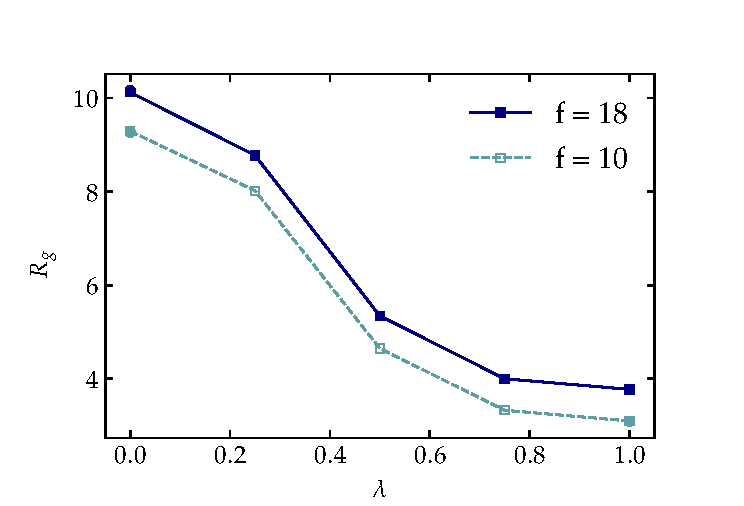
\includegraphics{figures/test_1.eps}
    \caption{Caption}
    \label{fig:test}
\end{figure}
\begin{figure}
    \centering
    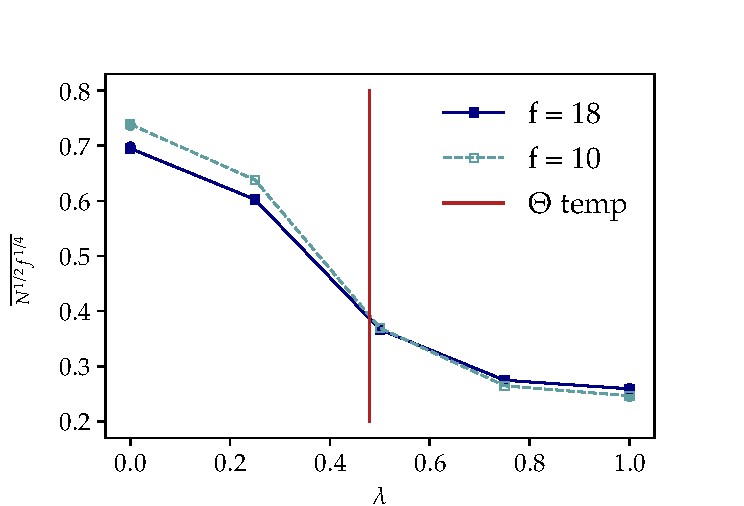
\includegraphics{figures/test_1_normalized.eps}
    \caption{Caption}
    \label{fig:tes:normal}
\end{figure}


